\documentclass[../main.tex]{subfiles}

\begin{document}

\section{Primer apartado}

En este apartado, se ha realizado la medida de latencia de interrupción con un osciloscopio, usando el módulo cuyo código fuente se nos proporcionaba en el directorio de prácticas de la asignatura. \cite{fuentes-modulo}. 

\subsection{Compilación e instalación del módulo}

Una vez descargados los fuentes del módulo, se ha procedido a su compilación. Para ello, tras renombrar el fichero \it{test-irq-latency.c} como \it{test\_irq\_latency.c}, ha bastado con seguir los pasos que se indicaban en el guión; se nos proporcionaba un \it{Makefile}, por lo que solo era necesario modificar el valor de ciertas variables de shell para que todo funcionase.

Una vez con el fichero \it{test\_irq\_latency.ko} generado, se ha instalado en la distribución, copiándolo en el directorio raiz de la partición \it{rootfs}.

\subsection{Preparación de las conexiones al osciloscopio}

El siguiente paso fue realizar las conexiones necesarias entre los pines de la BeagleBone y el osciloscopio. Una vez hechas, quedan tal que:

\begin{figure}[h]
\centering
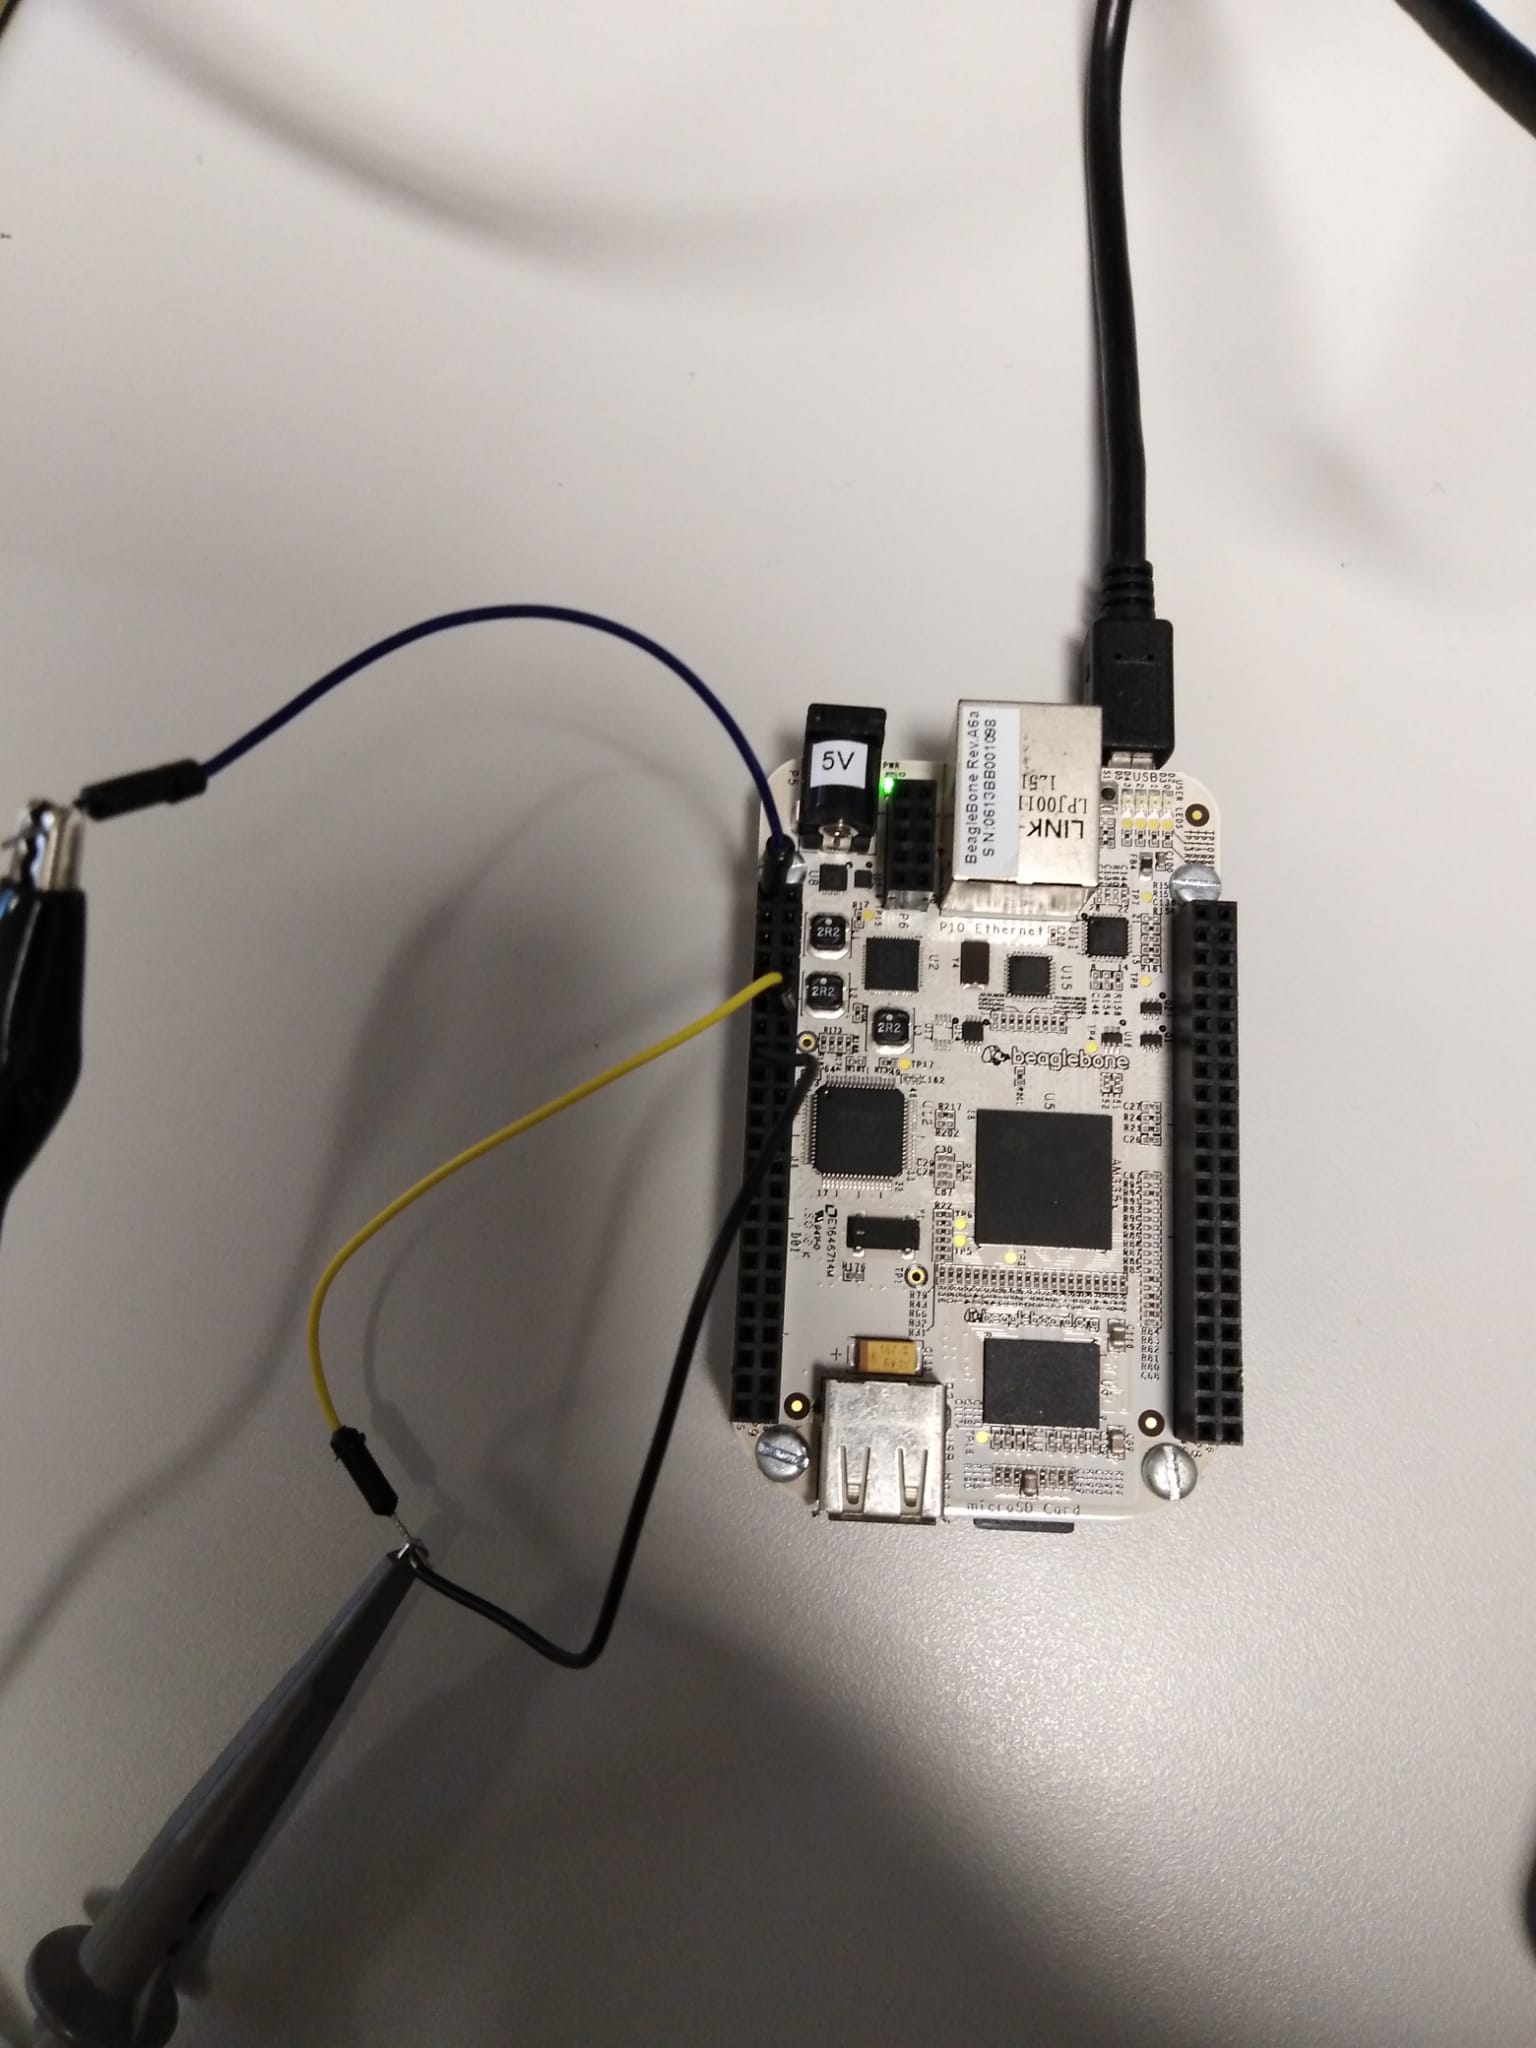
\includegraphics[width=0.5\textwidth]{imagenes/Apartado1-FotografiaPlaca.jpeg}
\caption{Fotografía a la placa con las conexiones necesarias al osciloscopio}
\end{figure}

En esta práctica se trabaja con el \it{espansion header P9}, que son los pines de la izquierda al colocar la placa como en la fotografía. Se puede observar cómo el pin 1, que es la tierra, está conectado a la tierra del osciloscopio, mientras los pines 12 y 15 están unidos entre sí y a la sonda del osciloscopio.

\subsection{Medición de la latencia de interrupción}

Una vez llegado este punto, se procede a medir la latencia de interrupción por software y con el osciloscopio.

Dentro de la distribución, se ejecuta \it{insmod test\_irq\_latency.ko}, que cargará el módulo y hará que se ejecute su función de init, \it{test\_irq\_latency\_init\_module}. En ella se empieza escribiendo en los registros de control de los pines P9/12 y P9/15, para que queden configurados como GPIOs (función \it{setup\_pinmux}, configura ambos pines en modo 7). Después, se solicita el uso de esos dos pines al kernel, y si todo transcurre sin problemas, al pin P9/15 se le asocia una IRQ, que tendrá como handler la función \it{test\_irq\_latency\_interrupt\_handler}. Después, se configura un timer para que ejecute la función \it{test\_irq\_latency\_timer\_handler} de manera periódica hasta que se cumpla un tiempo de expiración.

Tras ello, pasará lo siguiente: el pin P9/12 empieza teniendo un valor constante igual a 1, pero de manera periódica, el timer que se ha programado ejecuta la función \it{test\_irq\_latency\_timer\_handler}, y ésta permuta ese valor a 0. Por otra parte, cuando se detecta el valor 0 en el pin P9/15, salta la interrupción que éste tiene asociada, y es atendida por la función \it{test\_irq\_latency\_interrupt\_handler}, que pone el pin P9/12 a 1 de nuevo.

Además de eso, ambas funciones comparten un struct, que es global al módulo. Sirve, por ejemplo, para intercambiar información acerca de si la última permutación del valor del pin P9/12 ha causado una interrupción que ha sido atendida correctamente, y así detectar errores. También almacena variables como  \it{test\_count}, que es el contador de eventos generados, y sirve como condición de parada en las mediciones.

En el tiempo que transcurre hasta que se generan \it{NUM\_TESTS} eventos periódicos en el pin P9/12, se puede observar en el canal del osciloscopio lo siguiente:

\begin{figure}[h]
\centering
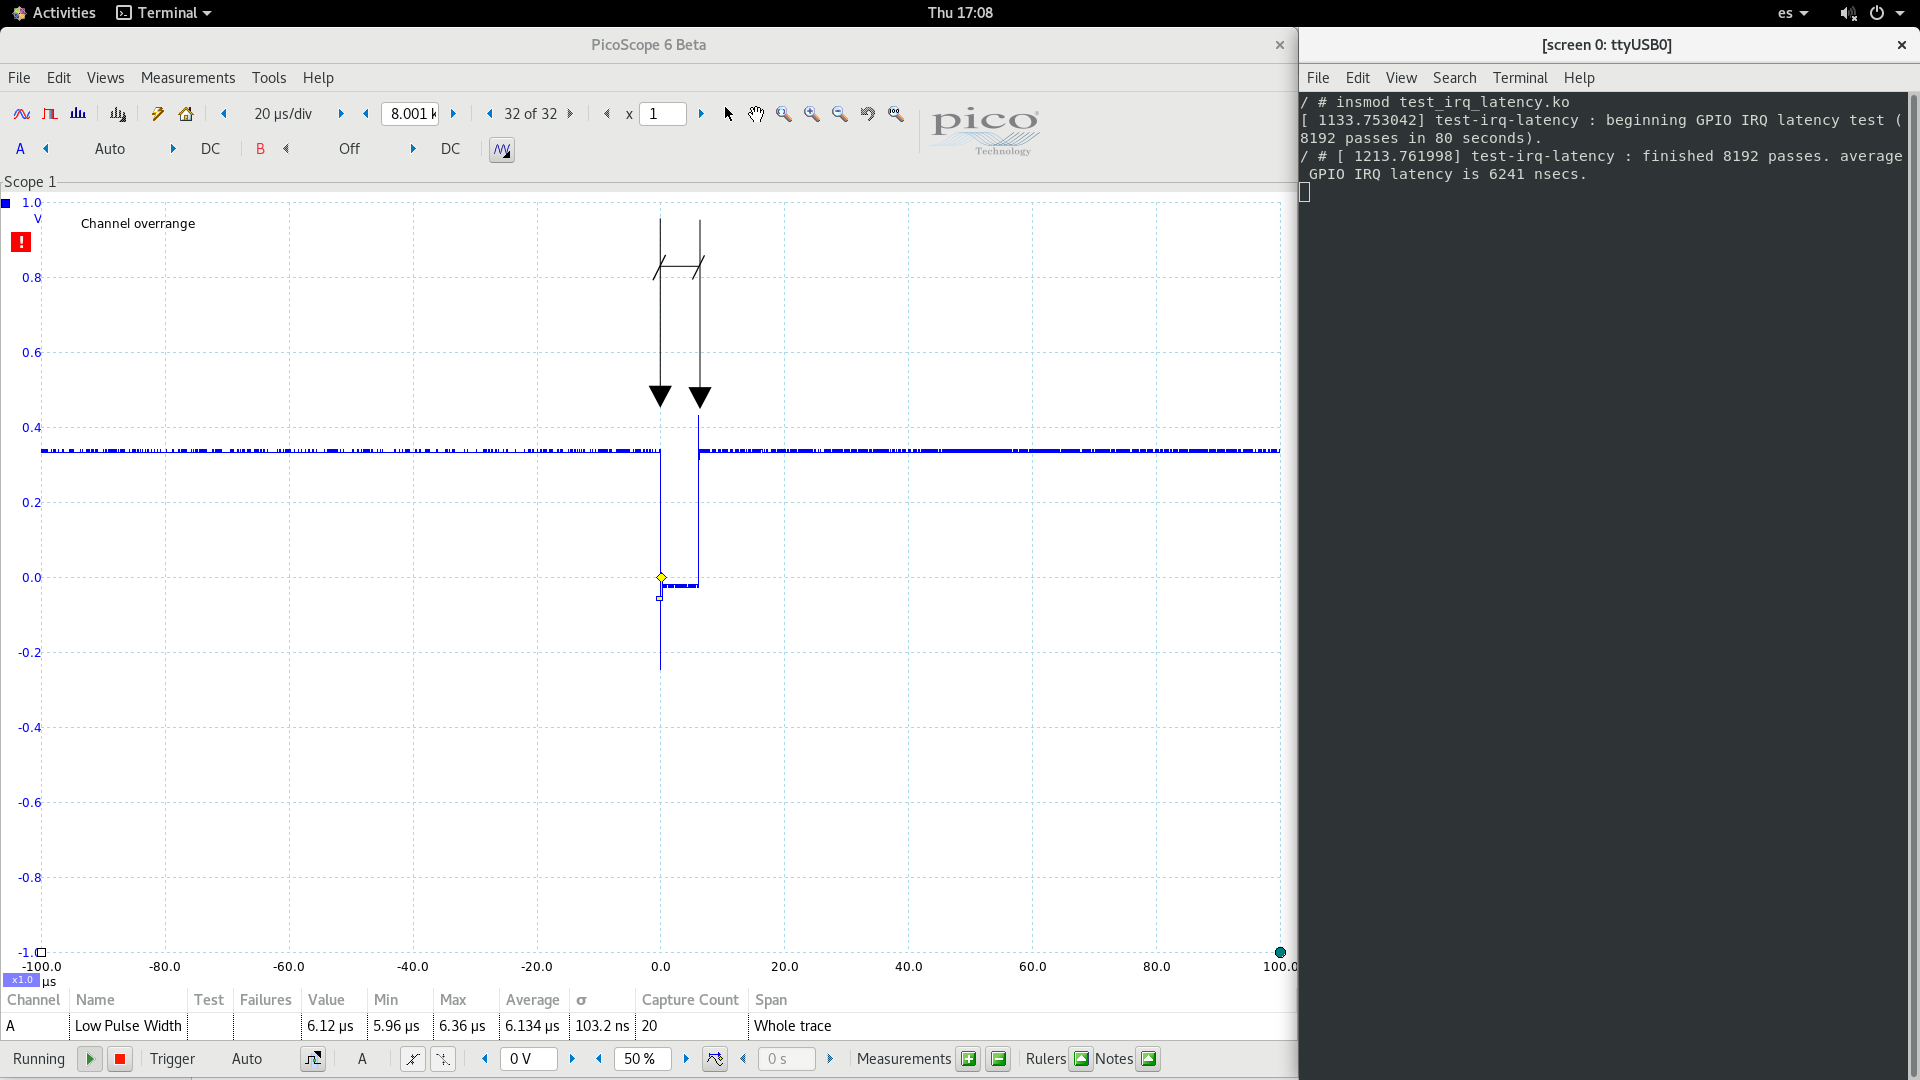
\includegraphics[width=1\textwidth]{imagenes/Apartado1-CapturaOsciloscopio.png}
\caption{Captura de pantalla del momento en el que terminan los eventos temporizados}
\end{figure}

Las dos flechas verticales indican el de tiempo que dura la latencia de interrupción, que es el tiempo que pasa desde que la función \it{test\_irq\_latency\_timer\_handler} pone a 0 el valor del pin P9/12 y la función \it{test\_irq\_latency\_interrupt\_handler} lo vuelve a poner a 1.

Cuando se superan los \it{NUM\_TESTS} eventos generados, la función \it{test\_irq\_latency\_timer\_handler} muestra por pantalla un mensaje con la latencia media que se ha medido por software. Como se puede observar en la figura, la medición hecha con el osciloscopio y la medición software son prácticamente iguales.

\subsection{Solución al problema de desmontaje del módulo}

El problema se producía al ejecutar \it{rmmod test\_irq\_latency.ko}, pues no se obtenía ningún mensaje, pero tampoco se desmontaba el módulo (ejecutando \it{lsmod} se podía comprobar que el módulo seguía montado).

La solución era ejecutar el comando sin la extensión en el nombre del módulo, es decir, ejecutar \it{rmmod test\_irq\_latency}. De esa forma, el módulo quedaba correctamente desmontado. 

Otra posible solución era hacer un reset de la placa, de forma que al volver a arrancar el sistema, el módulo ya no estuviese cargado.

\end{document}